\chapter{质谱法与原子光谱法}\label{ch:b2:mass-spec-atomic}

烟花因含锶盐而呈红色，含钡盐而呈绿色，含钠盐则呈黄色：火焰能把
原子转化为颜色各具特征、可用以辨认它们的光。质谱仪外观朴素得多，
它能称量单个分子，按同位素对其分类，并将分子打碎成若干片段；这些片段的质量可说明
分子是如何构成的。两种技术都回答“样品中有什么，含量多少？”这一问题，
所需样品量都极少：前者针对分子，后者针对元素。

\begin{omfigure}
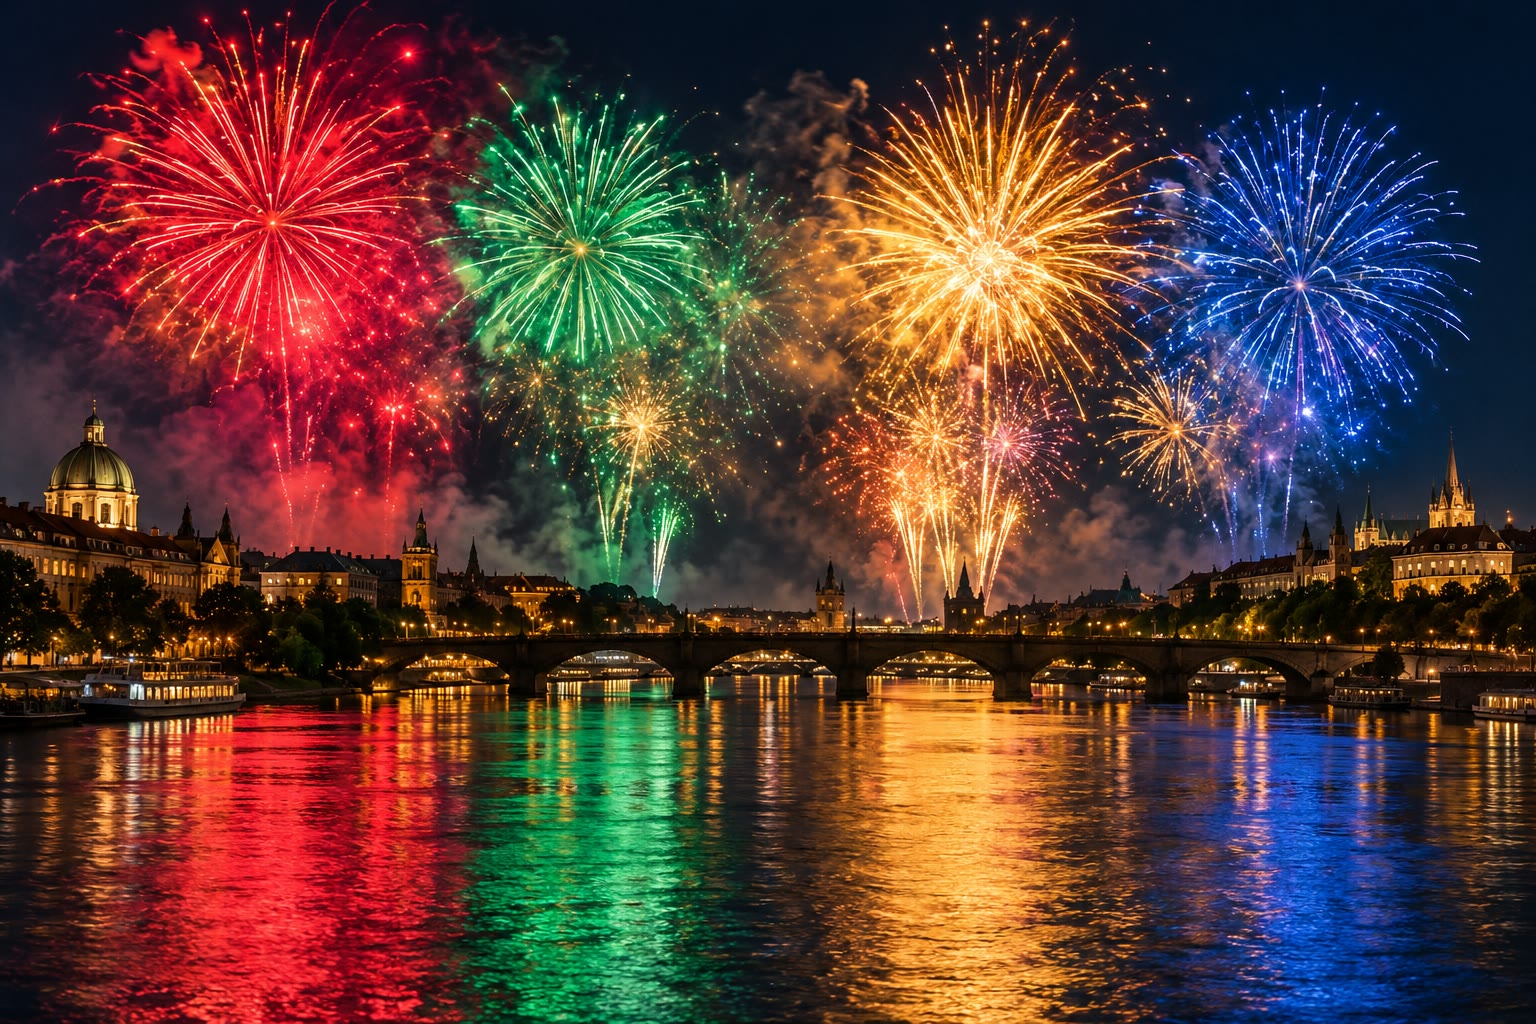
\includegraphics[width=0.58\linewidth]{images/book3/ai/b2-32-fireworks.jpg}

{\small 河面上空的烟花（示意图）。钠的黄色来自钠原子发出的光；
红色与绿色则主要来自火焰中生成的锶和钡的小分子。}
\end{omfigure}

\begin{recall}
第 1 册：同位素及其丰度。本科一年级分册：能级与
谱线、吸光度与比尔–朗伯定律、碳正离子与自由基、不饱和度。
\Cref{ch:b2:chromatography}：气相色谱法，常与质谱仪联用。
\end{recall}

\section{质谱仪}

\begin{definition}[质谱法]\label{def:b2:mass-spec-atomic:spectrum}
\emph{质谱法}\index{质谱法}把样品中的分子转化为气态离子，
将离子按其\emph{质荷比}\index{质荷比} $m/z$
（即以原子质量单位计的质量除以电荷数）分离并计数。
\emph{质谱图}\index{质谱图}以离子丰度对 $m/z$ 作图，通常以
相对强度表示；其中最强的峰记为 100，即\emph{基峰}\index{基峰}。
\end{definition}

质谱仪由三部分组成。离子源用于产生离子。在电子电离（EI）中，样品的蒸气
穿过能量为 \qty{70}{eV} 的电子束，电子将分子中的一个电子击出，
并使分子具有过剩能量，因而许多分子发生断裂。在电喷雾电离（ESI）中，溶液
从带电针头喷出；液滴蒸发时，分子带着一个额外质子
（或一个钠离子）逸出液滴并保持完整，是处理大而易碎分子的首选方法。随后，分析器对
离子加以分离，检测器对其计数。

\begin{omfigure}
\begin{tikzpicture}[x=1cm, y=1cm]
\draw[black!70, fill=omDef!10, rounded corners=2pt] (0,-0.6) rectangle (1.6,0.6);
\node[font=\small, align=center] at (0.8,0) {离子 \\源};
\draw[black!70] (2.0,-0.7) -- (2.0,0.7); \draw[black!70] (2.4,-0.7) -- (2.4,0.7);
\node[font=\footnotesize] at (2.2,1.0) {栅极，$U$};
\draw[black!70] (2.6,-0.5) rectangle (8.4,0.5);
\node[font=\small] at (5.6,0.8) {无场漂移管，长度 $L$};
\draw[black!70, fill=black!15] (8.5,-0.6) rectangle (8.8,0.6);
\node[font=\small, align=center] at (9.6,0) {检测器};
\foreach \x/\c in {3.4/omThm, 4.6/omDef, 6.3/omMeth}{\fill[\c] (\x,0) circle (0.1);}
\draw[->, thick] (6.6,0) -- (7.4,0);
\node[font=\footnotesize, align=center] at (5.5,-0.85) {轻离子飞在前，重离子落后};
\end{tikzpicture}
\par\vspace{4pt}

{\small 飞行时间分析器（示意图）。经同一电势差加速的离子
$U$ 加速后动能相同；在漂移管中，较轻的离子运动较快，
因而先到达检测器。}
\end{omfigure}

\begin{proposition}[飞行时间]\label{prop:b2:mass-spec-atomic:time-of-flight}
质量为 $m$、电荷为 $ze$ 的离子，从静止经电势差 $U$ 加速后，穿过
长度为 $L$ 的无场管，所用时间为
\begin{equation*}
t = L\sqrt{\frac{m}{2zeU}}:
\end{equation*}
飞行时间随 $m/z$ 的平方根增长。
\end{proposition}

\begin{proof}
由加速电场中的能量守恒得 $\tfrac12mv^2 = zeU$，故 $v = \sqrt{2zeU/m}$，
且离子以恒定速率穿过无场管：$t = L/v$。
\end{proof}

其他分析器以不同方式分离离子：四极杆一次只让某一 $m/z$ 的离子通过，
通过四根电极杆上的交变电压进行选择；磁扇形场使离子沿圆周偏转，圆周半径
取决于离子的动量。这些分析器测量的都只是 $m/z$；由 EI 产生的大多数离子只带一个
电荷，因此 $m/z$ 就等于其质量。

\section{分子离子}

\begin{definition}[分子离子与碎片离子]\label{def:b2:mass-spec-atomic:molecular-ion}
\emph{分子离子}\index{分子离子} $\mathrm M^{+\bullet}$ 是分子失去一个电子后形成的
自由基阳离子；其 $m/z$ 等于由丰度最高的同位素组成的分子的
摩尔质量。\emph{碎片离子}\index{碎片离子}由分子离子经
化学键断裂而来。
\end{definition}

分子离子给出分子质量，这是关于未知物的第一条信息。在电子电离中，分子离子有时很弱甚至
缺失，原因是其极易断裂；电喷雾电离给出 $[\mathrm M +
\mathrm H]^+$ 峰，比分子质量高一个单位，可用来确认。

\begin{definition}[氮规则]\label{def:b2:mass-spec-atomic:nitrogen-rule}
\emph{氮规则}\index{氮规则}指出：分子的标称质量（即其丰度最高的同位素的质量数之和）
为奇数，当且仅当其含奇数个氮
原子。
\end{definition}

\begin{proposition}[氮规则的有效性]\label{prop:b2:mass-spec-atomic:nitrogen-rule}
氮规则对所有不含未成对电子、由 C、H、N、O、S 和卤素构成的分子
均成立。
\end{proposition}

\begin{proof}
C（12）、N（14）、O（16）、S（32）的标称质量为偶数，H（1）及卤素（19、
35、79、127）。C、O、S 的化合价为偶数，H、N 及卤素的为奇数。在不含未成对电子的分子中，
每个键分别占用两端原子各一个化合价，因此所有化合价之和
为偶数，而奇数化合价原子的个数 $n_{\ce{H}} + n_{\ce{X}} + n_{\ce{N}}$ 为
偶数。标称质量的奇偶性与 $n_{\ce{H}} + n_{\ce{X}}$ 的相同，因而也与
$n_{\ce{N}}$ 的相同。
\end{proof}

\begin{definition}[同位素峰形]\label{def:b2:mass-spec-atomic:isotope-pattern}
离子的\emph{同位素峰形}\index{同位素峰形}是指一组峰，它们位于 $M$、$M+1$、
$M+2$、\dots\ 处，由含较重同位素的分子产生，
其强度与各同位素形式的丰度成正比。
\end{definition}

\begin{proposition}[$M+1$ 峰]\label{prop:b2:mass-spec-atomic:m-plus-one}
设离子含 $n_C$ 个碳原子，且不含其他具有显著 $+1$ 同位素的元素，
\begin{equation*}
\frac{I(M+1)}{I(M)} \approx n_C\,\frac{a_{13}}{a_{12}} \approx n_C \times 1.1~\%,
\end{equation*}
其中 $a_{12} = 0.989$、$a_{13} = 0.011$ 分别为两种碳同位素的物质的量分数。
% ledger: iso:C12, iso:C13
\end{proposition}

\begin{proof}
所有 $n_C$ 个碳原子均为 \ce{^{12}C} 的概率为 $a_{12}^{n_C}$；恰有一个为
\ce{^{13}C} 的概率为 $n_C\,a_{13}a_{12}^{n_C - 1}$（二项定律）。比值为 $n_C\,a_{13}/a_{12}$，而
其余贡献（两个 \ce{^{13}C}、\ce{^2H}、\ce{^{15}N}）
都要小一个约为 $a_{13}$ 量级或更小的因子。
\end{proof}

\begin{proposition}[氯和溴]\label{prop:b2:mass-spec-atomic:halogen-patterns}
设离子含 $p$ 个氯原子和 $q$ 个溴原子，则 $M$、$M+2$、$M+4$、\dots\ 处的强度
为展开式 $(a_{35} + a_{37}x)^p(a_{79} + a_{81}x)^q$ 中 $x$ 各次幂的系数，
$x$ 的每一次幂对应 2 个质量单位。取 $a_{35} = 0.758$、$a_{37} = 0.242$、$a_{79} = 0.5069$ 与
$a_{81} = 0.4931$，则一个氯原子给出 $M : M+2 \approx 3 : 1$，一个溴原子给出 $\approx 1 : 1$。
% ledger: iso:Cl35, iso:Cl37, iso:Br79, iso:Br81
\end{proposition}

\begin{proof}
每个卤素原子独立地为轻同位素或重同位素，后者使质量增加 2 个单位。含
$j$ 个重原子的概率即为各原子因子乘积中 $x^j$ 的系数，
即上述展开式（对每种元素应用二项定律）。
\end{proof}

\begin{omfigure}
\pgfplotsset{clu/.style={width=0.25\linewidth, height=3.3cm, ybar, bar width=5pt, ymin=0, ymax=118,
  xmin=-1.2, xmax=5.2, xtick={0,2,4}, xticklabels={$M$,$M\!+\!2$,$M\!+\!4$},
  tick label style={font=\tiny}, ytick=\empty, axis x line=bottom, axis y line=none,
  title style={font=\small, yshift=-4pt}, nodes near coords, nodes near coords style={font=\tiny},
  point meta=y, every node near coord/.append style={/pgf/number format/fixed, /pgf/number format/precision=0}}}
\begin{tikzpicture}
\begin{axis}[clu, title={Cl}]
\addplot[fill=omDef!55, draw=omDef, y filter/.expression={y==0 ? nan : y}] table[x=off, y=Cl] {figdata/out/bachelor-2-mass-spectra-a.dat};
\end{axis}
\end{tikzpicture}\hfill
\begin{tikzpicture}
\begin{axis}[clu, title={Cl$_2$}]
\addplot[fill=omDef!55, draw=omDef] table[x=off, y=Cl2] {figdata/out/bachelor-2-mass-spectra-a.dat};
\end{axis}
\end{tikzpicture}\hfill
\begin{tikzpicture}
\begin{axis}[clu, title={Br}]
\addplot[fill=omThm!45, draw=omThm, y filter/.expression={y==0 ? nan : y}] table[x=off, y=Br] {figdata/out/bachelor-2-mass-spectra-a.dat};
\end{axis}
\end{tikzpicture}\hfill
\begin{tikzpicture}
\begin{axis}[clu, title={Br$_2$}]
\addplot[fill=omThm!45, draw=omThm] table[x=off, y=Br2] {figdata/out/bachelor-2-mass-spectra-a.dat};
\end{axis}
\end{tikzpicture}\hfill
\begin{tikzpicture}
\begin{axis}[clu, title={氯溴}]
\addplot[fill=omMeth!45, draw=omMeth] table[x=off, y=ClBr] {figdata/out/bachelor-2-mass-spectra-a.dat};
\end{axis}
\end{tikzpicture}

{\small 含氯和溴的离子的同位素峰形，依据同位素
丰度计算（见\cref{prop:b2:mass-spec-atomic:halogen-patterns}）；每组中最强的峰强度
设为 100。峰形具有特征：一个氯为 3 : 1，一个溴为 1 : 1，
两个溴为 1 : 2 : 1。}
% figdata: bachelor-2/mass-spectra.py part a
\end{omfigure}

\begin{definition}[精确质量]\label{def:b2:mass-spec-atomic:exact-mass}
离子的\emph{单同位素质量}\index{单同位素质量}是其中最丰富同位素的精确质量之和
（\ce{^{12}C} 恰为 12，\ce{^1H} = 1.007825，\ce{^{16}O} = 15.994915，
\ce{^{14}N} = 14.003074 u）。\emph{高分辨质谱法}\index{高分辨质谱法}
可将 $m/z$ 测量到千分之几单位或更高精度，足以区分名义质量相同、
但化学式不同的离子。
% ledger: mass:C12, mass:H1, mass:O16, mass:N14
\end{definition}

\begin{proposition}[分辨本领]\label{prop:b2:mass-spec-atomic:resolving}
质量分别为 $m$ 和 $m + \Delta m$ 的两个离子能被分开，所需分析器的分辨本领至少为
$R = m/\Delta m$。名义质量为 28 时，分离 \ce{CO+}（27.9949）与 \ce{N2+}（28.0061）需要 $R
\approx 2.5 \times 10^3$；分离 \ce{N2+} 与 \ce{C2H4+}（28.0313）时，$R \approx 1.1 \times 10^3$。
\end{proposition}

\begin{proof}
分辨本领定义为 $m/\Delta m$，其中 $\Delta m$ 取分析器能分开的最小值。
精确质量由同位素质量算得：$12 + 15.994915$、$2 \times 14.003074$、$24 + 4 \times
1.007825$；于是 $28/(28.0061 - 27.9949) \approx 2.5 \times 10^3$ 与 $28/(28.0313 - 28.0061) \approx
1.1 \times 10^3$。
\end{proof}

\section{碎裂}

由 EI 产生的分子离子所携带的能量远超任何化学键断裂所需，它沿着
能生成最稳定生成物的途径断裂：稳定化的阳离子、小的稳定中性分子或
自由基。碎片可由 $M$ 的质量损失读出（\ce{CH3} 为 15，\ce{C2H5} 或 \ce{CHO} 为 29，
水为 18，CO 或乙烯为 28），也可由特征离子识别。

\begin{definition}[两种碎裂]\label{def:b2:mass-spec-atomic:fragmentation}
在\emph{$\alpha$-裂解}\index{$\alpha$-裂解}中，与
杂原子或羰基相邻的碳之间的键断裂，留下由杂原子孤电子对稳定化的阳离子（对酮为酰基正离子
$\mathrm{R{-}C{\equiv}O^+}$，对胺为亚胺正离子）。\emph{麦氏
重排}\index{麦氏重排}作用于羰基化合物时，将
$\gamma$ 碳上的氢转移到羰基氧上，并断裂 $\alpha$--$\beta$ 键，释放出一个烯烃和一个
烯醇自由基阳离子。
\end{definition}

\begin{omfigure}
\begin{tikzpicture}
\begin{axis}[width=0.48\linewidth, height=4.6cm, xmin=10, xmax=80, ymin=0, ymax=118,
  xlabel={$m/z$}, ylabel={相对强度}, label style={font=\small}, tick label style={font=\scriptsize},
  title={\small 2-丁酮}, ycomb, xtick={15,29,43,57,72}]
\addplot[omDef, thick] table[x=mz, y=I] {figdata/out/bachelor-2-mass-spectra-b.dat};
\node[font=\tiny, anchor=south] at (axis cs:43,100) {43};
\node[font=\tiny, anchor=south] at (axis cs:72,25) {72};
\node[font=\tiny, anchor=south] at (axis cs:57,8) {57};
\node[font=\tiny, anchor=south] at (axis cs:29,17) {29};
\end{axis}
\end{tikzpicture}\hfill
\begin{tikzpicture}
\begin{axis}[width=0.48\linewidth, height=4.6cm, xmin=10, xmax=140, ymin=0, ymax=118,
  xlabel={$m/z$}, ylabel={相对强度}, label style={font=\small}, tick label style={font=\scriptsize},
  title={\small 1-溴丙烷}, ycomb, xtick={27,43,79,107,122}]
\addplot[omThm, thick] table[x=mz, y=I] {figdata/out/bachelor-2-mass-spectra-c.dat};
\node[font=\tiny, anchor=south] at (axis cs:43,100) {43};
\node[font=\tiny, anchor=south] at (axis cs:123,9) {122, 124};
\node[font=\tiny, anchor=south] at (axis cs:27,26) {27};
\node[font=\tiny, anchor=south east] at (axis cs:40.5,31) {41};
\end{axis}
\end{tikzpicture}

{\small 电子电离谱图（NIST WebBook 数据）。2-丁酮：分子离子位于 72；
$\alpha$-裂解生成酰基正离子 \ce{CH3CO+}（43，基峰）和 \ce{C2H5CO+}（57）。1-溴丙烷：
分子离子为 122 与 124 处的 1 : 1 双峰（\ce{^{79}Br}、\ce{^{81}Br}）；失去溴原子后
留下 \ce{C3H7+}，位于 43，即基峰。}
% figdata: bachelor-2/mass-spectra.py parts b, c
% ledger: ms:butanone, ms:bromopropane
\end{omfigure}

\begin{omfigure}
\setchemfig{atom sep=1.8em}
\schemestart
\chemfig{[:-30]\chemabove{O}{\scriptstyle +\bullet}?[a]=[:-90]C(-[:-150]H_3C)-[:-30]CH_2-[:30]CH_2-[:90]CH_2-[:150]H?[a,1,{dash pattern=on 1pt off 1.5pt}]}
\arrow{->}[,1.0]
\chemfig{CH_2=C(-[2]OH)-CH_3}\,$^{+\bullet}$
\+
\chemfig{CH_2=CH_2}
\schemestop
\par\vspace{6pt}

{\small 戊-2-酮的麦氏重排，以其六元环状结构表示：
$\gamma$ 碳上的氢转移至氧原子，$\alpha$--$\beta$ 键断裂，
乙烯离去，丙酮的烯醇自由基阳离子保留在 $m/z$ 58 处。}
\end{omfigure}

\begin{proposition}[麦氏重排的条件]\label{prop:b2:mass-spec-atomic:mclafferty}
麦氏重排要求 $\gamma$ 碳上有氢。它释放出一个烯烃，并留下
一个自由基阳离子，其质量与分子质量的奇偶性相同（对不含
氮的化合物为偶数）。
\end{proposition}

\begin{proof}[论证]
氢经由一个六元环状结构转移，该结构由氧原子、羰基碳、
$\alpha$、$\beta$、$\gamma$ 碳及氢原子自身组成：只有 $\gamma$ 位氢
能无张力地到达氧原子。生成的离子保留羰基、$\alpha$ 碳及
被转移的氢；离去的是烯烃，一种质量为偶数的中性分子，故离子
保持 $M$ 的奇偶性，这使其有别于简单裂解生成的奇数质量阳离子。
\end{proof}

\begin{method}[读取质谱图]\label{met:b2:mass-spec-atomic:read-ms}
\begin{enumerate}
  \item 找出分子离子（主峰群中最高的 $m/z$，其下方应有合理的丢失峰）。
  \item 读取其同位素峰形：Cl、Br、S；$M+1$ 峰给出碳原子数。
  \item 应用氮规则，提出分子式及其不饱和度。
  \item 读取相对于 $M$ 的丢失峰及特征离子（43 \ce{CH3CO+} 或 \ce{C3H7+}，77
        \ce{C6H5+}、91 \ce{C7H7+}、105 \ce{C6H5CO+}）；寻找偶数质量的麦氏重排离子。
  \item 提出结构，并核对每一个重要峰均可得到解释。
\end{enumerate}
\end{method}

\section{原子光谱法}

原子没有振动与转动，其光谱是尖锐的谱线，每一次电子能级间的跃迁
对应一条谱线，谱线波长是该元素特有的。钠火焰的黄色来自
一对谱线，分别位于 \qty{589.0}{nm} 与 \qty{589.6}{nm}；锂的深红色来自位于 \qty{670.8}{nm} 处的一条谱线；
锶原子最强的谱线位于 \qty{460.7}{nm}，钡离子的最强谱线位于
\qty{455.4}{nm}，处于蓝色区段。烟花中的红色与绿色主要来自这些金属的分子，
而非其原子。
% ledger: asd:NaD2, asd:NaD1, asd:Li671, asd:Sr461, asd:Ba455

\begin{definition}[原子光谱法]\label{def:b2:mass-spec-atomic:atomic}
在\emph{原子发射光谱法}\index{原子发射光谱法}中，样品被原子化并
在火焰或等离子体中激发，并测量该元素某一发射谱线的强度。在
\emph{原子吸收光谱法}\index{原子吸收光谱法}（AAS）中，样品
在火焰或石墨炉中原子化，并在共振线处测量原子的吸光度，
该共振线由\emph{空心阴极灯}\index{空心阴极灯}发出，其阴极由
该元素本身制成。在\emph{电感耦合等离子体}\index{电感耦合等离子体}（ICP）中，氩气
在射频场作用下被加热至数千开尔文，使样品原子化并电离；该
等离子体可接入发射光谱仪（ICP-OES）或质谱仪（ICP-MS）。
\end{definition}

\begin{omfigure}
\begin{tikzpicture}[x=1cm, y=1cm, box/.style={draw=black!70, rounded corners=2pt, fill=white,
  font=\small, align=center, minimum height=0.8cm, inner sep=3pt}]
\node[box] (lamp) at (0,0) {空心阴极 \\灯 (Cu)};
\shade[top color=omThm!60, bottom color=omThm!10] (2.6,-0.25) -- (3.3,-0.25) -- (3.15,0.75) -- (2.75,0.75) -- cycle;
\draw[black!70, fill=black!15] (2.4,-0.45) rectangle (3.5,-0.25);
\node[font=\footnotesize] at (2.95,-0.75) {火焰（原子）};
\node[box] (mono) at (6.1,0) {单色 \\仪};
\node[box] (det) at (8.5,0) {检测器};
\node[box] (data) at (10.8,0) {吸光度};
\draw[->, thick, omDef] (lamp.east) -- (mono.west);
\draw[->, thick] (mono) -- (det); \draw[->, thick] (det) -- (data);
\node[font=\footnotesize, omDef] at (4.4,0.3) {$I_0 \to I$};
\end{tikzpicture}
\par\vspace{4pt}

{\small 原子吸收光谱仪示意图。灯发出铜本身的谱线，其中
包括位于 \qty{324.75}{nm} 处的共振线；火焰中的铜原子吸收该谱线，
单色仪将该谱线分离出来，供检测器测量。}
% ledger: asd:Cu325
\end{omfigure}

\begin{proposition}[原子吸收是定量的]\label{prop:b2:mass-spec-atomic:aas}
在一定浓度范围内，在共振线处测得的吸光度
与喷入火焰的溶液中该元素的浓度成正比。
\end{proposition}

\admitted

这就是本科一年级分册中比尔–朗伯定律在自由原子上的应用：火焰将一定比例的
溶液转化为原子，而灯的谱线比吸收线窄，可视为单色光。
在高浓度时谱线会饱和，标准曲线发生弯曲，
因此需要检验工作范围。

\begin{method}[原子吸收测量的校准]\label{met:b2:mass-spec-atomic:aas-calibration}
\begin{enumerate}
  \item 配制一个空白样和四至五个标准样，覆盖预期的浓度范围，
        其酸基体与样品相同。
  \item 测量它们在所选谱线处的吸光度；拟合 $A = a\,c$（或 $A = a\,c + b$）；
        检验线性。
  \item 测量样品，必要时稀释至落入工作范围内；计算 $c = (A - b)/a$。
  \item 测定结束时再测量一个标准样以检查漂移；对每一次稀释进行校正。
\end{enumerate}
\end{method}

电感耦合等离子体质谱（ICP-MS）的检出浓度最低，但其离子在质量上可能与标称质量相同的其他离子相重叠：
等离子气中的 \ce{^{40}Ar^{16}O+} 落在 \ce{^{56}Fe+} 上，\ce{^{40}Ar+} 落在
\ce{^{40}Ca+} 上。使用高分辨分析器、碰撞池或待测物的另一种同位素，
可以消除这种干扰。检出限及其测定方法，
将在\cref{ch:b2:measurement-statistics}中讨论。

\begin{history}[称量原子，看见元素]
\begin{minipage}[t]{0.17\linewidth}
\vspace{0pt}
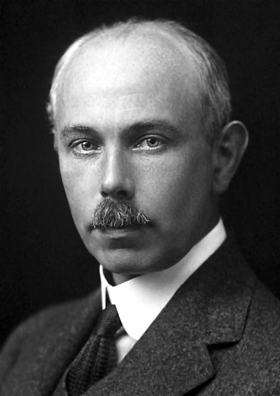
\includegraphics[width=\linewidth]{images/book3/aston.jpg}
\end{minipage}\hspace{0.02\linewidth}%
\begin{minipage}[t]{0.24\linewidth}
\vspace{0pt}
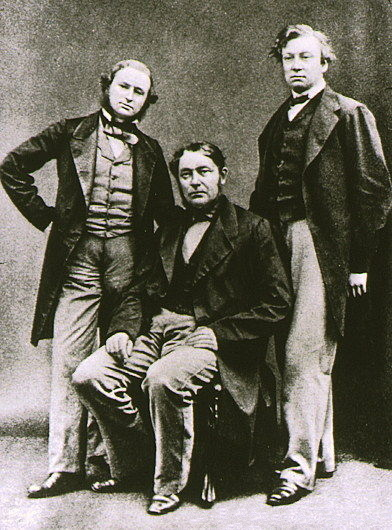
\includegraphics[width=\linewidth]{images/book3/kirchhoff-bunsen.jpg}
\end{minipage}\hfill
\begin{minipage}[t]{0.54\linewidth}
\vspace{0pt}
基尔霍夫与本生约于 1860 年指出，每种元素在火焰中都给出其特有的谱线，
并借助未知谱线发现了铯和铷。弗朗西斯·阿斯顿的质谱仪（1919 年）表明，
大多数元素都是同位素的混合物；他因此获得了 1922 年诺贝尔化学奖。
（照片：Aston，作者不详，公有领域；Kirchhoff、Bunsen 与 Henry Roscoe 摄于 1862 年，取自
罗斯科的收藏，公有领域；维基共享资源。）
\end{minipage}
\end{history}

\section{练习}

\begin{exercise}[$\star$]\label{exo:b2:mass-spec-atomic:1}
求下列各项的 $m/z$：苯 \ce{C6H6} 的分子离子；带两个电荷、质量为 \qty{400}{u} 的离子；
电喷雾形成的咖啡因质子化分子（\ce{C8H10N4O2}，标称质量 194）。
\end{exercise}

\begin{exercise}[$\star$]\label{exo:b2:mass-spec-atomic:2}
某化合物由 C、H、N、O 组成，其分子离子的 $m/z$ 为 73。关于其中的氮原子，能得出什么结论？
提出一个化学式。
\end{exercise}

\begin{exercise}[$\star$]\label{exo:b2:mass-spec-atomic:3}
某分子离子簇中两峰相隔两个质量单位，高度几乎相等；另一簇中两峰相隔两个质量单位，
强度比为 3 : 1。这是哪些卤素？
\end{exercise}

\begin{exercise}[$\star$]\label{exo:b2:mass-spec-atomic:4}
某盐使火焰呈黄色，另一种盐使火焰呈深红色。确定这些元素，
并给出其谱线的波长。
\end{exercise}

\begin{exercise}[$\star\star$]\label{exo:b2:mass-spec-atomic:5}
某烃在 $M$ 处为 100 \%，在 $M+1$ 处为 6.7 \%。它含有多少个碳原子？
\end{exercise}

\begin{exercise}[$\star\star$]\label{exo:b2:mass-spec-atomic:6}
计算 \ce{CO}、\ce{N2} 和 \ce{C2H4} 的精确质量，
以及分离每一对分子所需的分辨本领。
\end{exercise}

\begin{exercise}[$\star\star$]\label{exo:b2:mass-spec-atomic:7}
戊-3-酮的 EI 质谱在 86、57（基峰）和 29 处有峰。指出各峰的归属。
\end{exercise}

\begin{exercise}[$\star\star$]\label{exo:b2:mass-spec-atomic:8}
戊-2-酮的质谱在 86、71、58 和 43（基峰）处有峰。指出各峰的归属，
并说明为何戊-3-酮在 58 处只有很小的峰。
\end{exercise}

\begin{exercise}[$\star\star$]\label{exo:b2:mass-spec-atomic:9}
铜标准样的浓度分别为 1.0、2.0、3.0 和 \qty{4.0}{mg/L}，吸光度依次为 0.052、0.104、0.155 和 0.207；
某样品的吸光度为 0.128（练习数据）。计算其中铜的浓度。
\end{exercise}

\begin{exercise}[$\star\star\star$]\label{exo:b2:mass-spec-atomic:10}
在飞行时间分析器中，$L = \qty{1.00}{m}$，$U = \qty{20.0}{kV}$。计算
质量为 \qty{1000}{u} 的单电荷离子的飞行时间，以及它与质量为 \qty{1001}{u} 的离子之间的时间间隔。
\end{exercise}

\begin{exercise}[$\star\star\star$]\label{exo:b2:mass-spec-atomic:11}
计算二氯甲烷 \ce{CH2Cl2} 的分子离子簇，
给出各 $m/z$ 值及相对强度。
\end{exercise}

\begin{exercise}[$\star\star\star$]\label{exo:b2:mass-spec-atomic:12}
在 ICP-MS 中，\ce{^{40}Ar^{16}O+} 干扰 \ce{^{56}Fe+}。计算分离二者所需的分辨本领，
并提出另一种解决办法。
\end{exercise}

\section{问题：未知卤化物}

\begin{problem}[{周末问题——含氯和溴的分子离子簇、碳原子数、
碎片，以及逐峰核对的结构}]
\label{pb:b2:mass-spec-atomic:1}
一种无色液体经气相色谱洗脱后呈单一色谱峰，给出如下 EI 质谱（NIST
WebBook 数据）。主要峰（$m/z$：相对强度）：156：14.5；157：0.5；158：18.6；159：0.6；160：
4.4；107：6.7；109：6.3；93：3.3；95：2.9；77：59；79：18.7；76：39.5；49：12.9；51：4.3；41：100；39：
26.2；27：24.6。同位素丰度：\ce{^{35}Cl} 0.758、\ce{^{37}Cl} 0.242、\ce{^{79}Br} 0.5069、
\ce{^{81}Br} 0.4931、\ce{^{12}C} 0.989、\ce{^{13}C} 0.011。
% ledger: ms:bromochloropropane, iso:Cl35, iso:Cl37, iso:Br79, iso:Br81, iso:C12, iso:C13, mass:C12, mass:H1, mass:Br79, mass:Cl35

\begin{center}
\begin{tikzpicture}
\begin{axis}[width=0.8\linewidth, height=4.6cm, xmin=20, xmax=170, ymin=0, ymax=112,
  xlabel={$m/z$}, ylabel={相对强度}, label style={font=\small},
  tick label style={font=\scriptsize}, ycomb, xtick={27,41,49,77,93,107,122,156}]
\addplot[omDef, thick] table[x=mz, y=I] {figdata/out/bachelor-2-mass-spectra-d.dat};
\end{axis}
\end{tikzpicture}
\end{center}
% figdata: bachelor-2/mass-spectra.py part d

\medskip
\noindent\textbf{第一部分——分子离子。}
\begin{enumerate}
  \item 哪些峰构成分子离子簇？为什么它不是单一峰？
  \item 间隔为 2 的三峰簇提示存在哪些卤素？
  \item 最轻同位素形式的标称质量是多少？
  \item 氮规则说明了什么？
  \item 减去一个 \ce{^{79}Br} 和一个 \ce{^{35}Cl}，剩余部分的质量是多少，
        哪种烃类碎片具有该质量？
  \item 提出分子式，并给出其不饱和度。
\end{enumerate}

\medskip
\noindent\textbf{第二部分——碳原子数与精确质量。}
\begin{enumerate}[resume]
  \item 由 157/156 的比值估算碳原子数。
  \item 为什么此处的估算只是粗略的？
  \item 哪些同位素形式对 158 处的峰有贡献？
  \item 计算分子离子的单同位素质量。
  \item \ce{C10H20O} 的标称质量同样为 156（精确质量 156.151）。要分开这两种离子，
        需要多大的分辨本领？
  \item 含 C=C 键且卤素种类相同的化合物，其分子离子的标称质量
        是否会不同？
\end{enumerate}

\medskip
\noindent\textbf{第三部分——碎片。}
\begin{enumerate}[resume]
  \item 77/79 这一对峰的强度比为 3 : 1。失去了哪个原子，所得离子是什么？
  \item 解释 76 处的峰。
  \item 指认 41 处的基峰。
  \item 指认 49/51 这一对峰。
  \item 指认 93/95 和 107/109 两对峰。
  \item 为什么溴原子比氯原子更容易失去？
  \item 1-溴-1-氯丙烷会在 127、129 和 131 处给出 \ce{CHBrCl+}，质谱是否支持
        这一结构？
\end{enumerate}

\medskip
\noindent\textbf{第四部分——结构。}
\begin{enumerate}[resume]
  \item 提出结构。
  \item 检验该结构能否解释表中列出的每一个峰。
  \item 能否发生麦氏重排？为什么？
  \item 画出在 $m/z$ 63/65 处给出强峰、而在 49/51 处无峰的同分异构体。
  \item 哪些同位素形式构成 160 处的峰？
  \item 由同位素丰度，计算含一个氯和一个溴时 $M$、$M+2$ 和 $M+4$ 峰的比值，
        并将其与质谱进行比较。
\end{enumerate}
\end{problem}
